\documentclass{article}
\usepackage[utf8]{inputenc}
\usepackage{graphicx}
\usepackage{geometry}
\usepackage{hyperref}
\hypersetup{
    colorlinks,
    citecolor=black,
    filecolor=black,
    linkcolor=black,
    urlcolor=black
}

 \geometry{
 a4paper,
 left=30mm,
 right=30mm,
 top=30mm,
 }

\graphicspath{ {images/} }

%----------------------------------------------------------------------------------------
%	TITLE PAGE
%----------------------------------------------------------------------------------------

\newcommand*{\titleGP}{\begingroup
		\begin{figure}[t]
			\centering
			
\includegraphics[width=350px]{fortran-design-srs/images/UP_Logo.PNG}
		\end{figure}
\centering 
\vspace*{\baselineskip}

\rule{\textwidth}{1.6pt}\vspace*{-\baselineskip}\vspace*{2pt}
\rule{\textwidth}{0.4pt}\\[\baselineskip]

{\LARGE NavUP\\ [0.3\baselineskip] Architectural Requirements Specifications and Design } \\ [0.2\baselineskip]
\rule{\textwidth}{0.4pt}\vspace*{-\baselineskip}\vspace{3.2pt}
\rule{\textwidth}{1.6pt}\\[\baselineskip] %

% \scshape %
% A concise specification on the functional requirements  \\
% and use cases of NavUP \\[\baselineskip]

% \vspace*{2\baselineskip}

Compiled By \\[\baselineskip]
{\Large Andries Jacobus du Plooy - u15226183 \\ Joseph Phutjane Letsoalo - u15043844 \\ Mathapelo Matabane - u12206522 \\ Munyaradzi Mpofu - u15071830\\ Ritesh Doolabh - u15075754 \\ Midhun John Cheriyan - u17308632\par}

\bigskip
\bigskip

 	GitHub Repository:  
 	\href{https://github.com/RitzDoolabh/COS301-Team_Fortran}{COS 301 Team Fortran GitHub Repository(Phase 2)}




 

\vfill


{\scshape 2017} \\[0.3\baselineskip]
{\large TEAM FORTRAN}\par

\endgroup}

\begin{document}

\titleGP
\newpage


\begin{abstract}
\noindent This documentation covers all the design requirements for the NavUP system, this includes System's External Requirements Performance Requirements, Technology choices and Design Constraints, to name a few. Furthermore, the documentation brings to mind the appropriate design patterns to implement to construct the system.
\end{abstract}

\newpage
\tableofcontents

\newpage
\section{Introduction}
Information about the activities, points of interest and venues on campus is not
readily available to employees, students and visitors to the UP campus. This is
especially a problem at the beginning of the academic year when thousands of new
students come to campus to attend regular lectures and on open days when large
numbers of visitors have to find their way to exhibitions and service points.

\subsection{Purpose}
NavUP is aimed at providing access to a wealth of information about campus
activities, points of interest and venues via the campus WiFi network. The information
should be accessible using smart devices. Users should be able to use the
information to navigate on campus and be informed about activities and facts of their
interest.
\subsection{Scope}
The core of the system is a navigation tool which is enriched with functionality
receiving information of interest.

\section{References}
Goldman, J.L., Abraham, G. and Song, I. (1998) Generating Software Requirements Specification (IEEE Std. 830 1998) document with Use Cases. \\ Available at: http://www.pages.drexel.edu/~sga72/docs/SRSwithUseCases.pdf \\(Accessed: 24 February 2017).\\
\noindent Singh, E., Pieterse, V., Omeleze, S., Theunissen, M. (2017) 2017 Class Project NavUP. Available at: http://www.cs.up.ac.za/courses/COS301/NavUPRequirementsSpecification.pdf (Accessed: 27 February 2017).\\ 
\newpage

\section{External Interface Requirements}
\subsection{User Interface}


The Notifications subsystem will allow for notifications to be pushed to registered users in the form of E-mails. The E-mails will have a descriptive subject associated with it and will be accessible from any device that allows a form of e-mail service.
The subsystem will allow for notifications to be pushed to registered users in the form of SMS's. the SMS's will only have a senders name which will indicate the type of notification and the SMS's content will then go on to expand on the notifications description.
The subsystem will interact with users mostly on a cellular device and a color screen will be required to get the most out of the application in terms of the E-mail service, SMS's on the other hand are a vital part of most cellular devices and in most cases no extra functionality is required.

The system must be able to help the user locate buildings by the use of display, navigate and select functions over the system's built GUI.
The system shall provide help options to the user when locating a certain POI.

\bigskip
The interface for the Users module will serve as the first impression of the application, as it is the very first screen which the user will encounter upon making use of the application. The initial interface should be a log in page. In addition, the log in page should provide an option for an unregistered user to register. The registration option should provide a registration page for the user to enter and submit their registration details. Once a user is logged in, there should be links to various other system interfaces, such as Notifications, Navigation, Points of Interests, Events and Fitness. The user should have a profile page on which they may edit their profile details, such as their email address and user name. The profile page should also provide an option to delete the user profile.

\subsection{Software Interface}

In regard to the notifications subsystem, the application will require an e-mail and SMS application on the device of choice in order to receive notifications of this type.
The subsystem will need to have access to a database of users such that they can be added to the user lists for the particular type of notification/s of their preference. These lists will then be referenced when the notifications are being sent to the users. The subsystem will also need to interact with all the various other notifying modules that may want to send out information to the users of the application.

A programmatic interface for operations such as adding locations, modifying locations, deleting locations is required.


The user subsystem will need to have access to the user data inside the database. This will be for the purpose of storing the information of newly registered users, and retrieving user credentials for login purposes, etc. The user subsystem will interact with the notifications subsystem. The application will provide the functionality for users to receive various notifications through the notifications module, therefore there should be an appropriate form of communication between these two modules to facilitate this interaction. Interaction will occur between the user subsystem and the events subsystem. The application will allow a user to view events and maintain an events schedule, therefore the user module should have access to all informations related to events. Interaction will occur between the user and the point of interest module. Each user on the system will have the option to add a list of locations to their favorites list. This will require for the user module to have access to all of the location information on the system.

\subsection{Hardware Interface}

The application will mostly be used on mobile devices, and the interface should support mobile device screens which are between 4 and 10 inches in size. The application will also have a web interface which can be accessed through laptop computers, therefore the interface should also support laptop screens.

\bigskip
With the use of most cellular devices, a color screen will be required for the use of e-mails and the device must in all cases be able to display information in a way that is understandable by the user.
The device must have the appropriate hardware in place to allow a form of data connection between itself and the Internet.
The system needs a database of all the WI-FI hot spots around the campus to map out the location or each Point of Interest. Moreover, the system must update information pertaining to points of interest.

\subsection{Communication Interface}

The system will make use of a database in order to store all of the information required by the application's various modules. TCP (Transmission Control Protocol) will be used for any database communication within the system. The application itself will need to communicate with the server in order to request various services. HTTP (Hypertext Transfer Protocol) will be the main protocol used for communication between the application and the server. The application will have the functionality to send push notifications in the form of emails and sms. The SMTP (Simple Mail Transfer Protocol) will be used for any communication which occurs via email, and the Short Message Service protocol will be used for sms communication.


The Notifications subsystem will need to communicate with any other subsystem that wishes to create and send out notifications to the users.
The subsystem will need to communicate with an automated E-Mail service to send out the mass e-mails to the users. Each notifying module will have access to its own instance of the notification subsystem to prevent any notifications from different notifying modules causing any conflict, and this also allows for no waiting period between creating and sending of notifications. They will be delivered in real time.
The subsystem will need to communicate with an automated SMS service to send out the mass SMS's to the users. Each notifying module will have access to its own instance of the notification subsystem to prevent any notifications from different notifying modules causing any conflict, and this also allows for no waiting period between creating and sending of notifications. They will be delivered in real time.
The users will need to have the appropriate communications interfaces available to allow them to receive notifications. This would include a working cellphone SIM card with a registered cellphone number and/or a working e-mail account that is accessible on a device with a data connection of some form.

\newpage
\section{System Features - Modules}

\subsection{User}
\subsubsection{Scope}
The user management module is responsible for maintaining information about the registered
users of the system, including the authority levels of each user. Administrators can
manage information about venues and activities whilst users who have signed up
may request services from the various modules and persist private information
related to particular services.\newline
No information is stored for the guest user. When accessing the service, the user
assumes the guest role without being logged in. The guest user may use public
services and my register or log in.
When a user is registered, the fields shown in the domain model are stored for the
user using a unique automatically assigned ID. The user provides all other fields. The
password should be stored in encrypted format. The user may change the value of
any of the fields of his own record except the value of the isAdmin field.
The only difference between a User and an Admin is the value of the isAdmin field.
Only Admin users may change the value of the isAdmin field of other users.
There are three types of users: Admin, User and Guest.

	\begin{figure}[h!]
      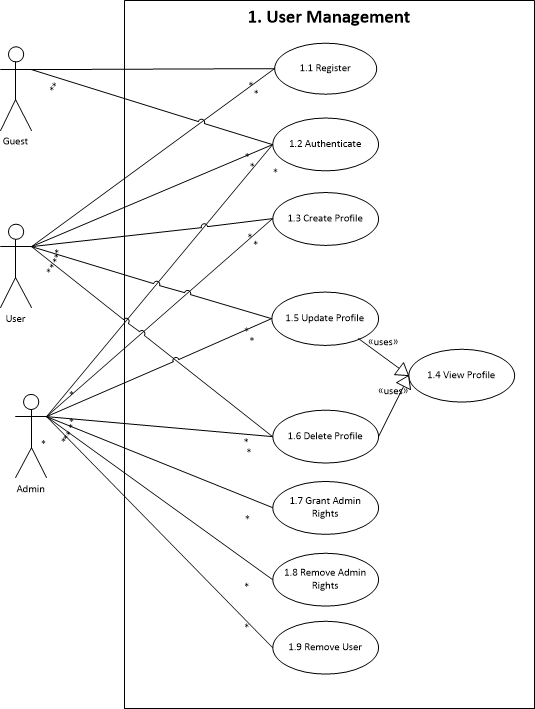
\includegraphics[width=\textwidth]{fortran-design-srs/images/User_Subsystem_Use_Case_Diagram.png}
      \caption{User Use Case Diagram Diagram}
    \end{figure}

	\clearpage
	
\subsubsection{Design details}

	\begin{figure}[h!]
      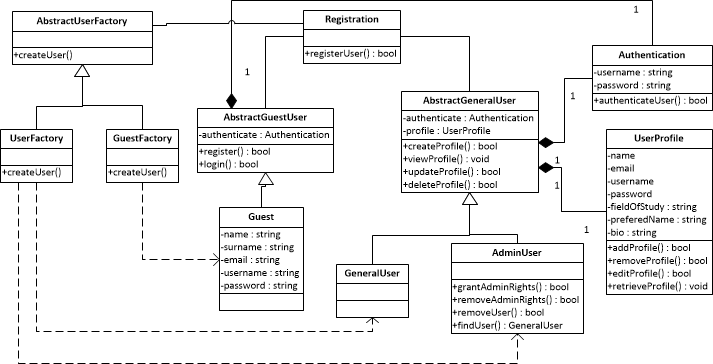
\includegraphics[width=\textwidth]{fortran-design-srs/images/User_Subsystem_Class_Diagram.png}
      \caption{User Class Diagram}
    \end{figure}
    
    \begin{flushleft}
    
    For the user subsystem, the Abstract Factory design pattern was used. The main reasoning behind this decision is that abstract factory is a creational pattern which can be used to create objects which are related to one another without having to specify their classes. This will facilitate the creation of 3 different types of users within the system, namely the guest users, general users, and administrator users, with each type of user having certain functionality which is not common to other user types.
    
     \bigskip
     
    Registration : Client

AbstractUserFactory : Abstract Factory

GuestFactory / UserFactory : Concrete Factory

AbstractGeneralUser / AbstractGuestUser : Abstract Product

GuestUser / GeneralUser / AdminUser : Concrete Product

\end{flushleft}

	\begin{figure}[h!]
      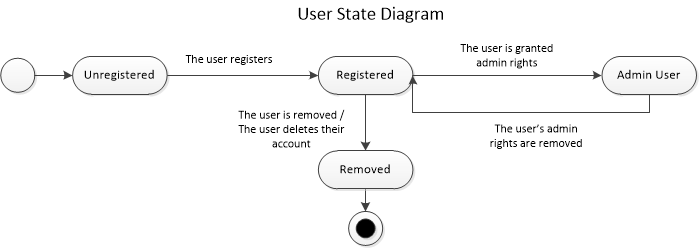
\includegraphics[width=\textwidth]{fortran-design-srs/images/User_State_Diagram.png}
      \caption{User State Diagram}
    \end{figure}

	\begin{figure}[h!]
      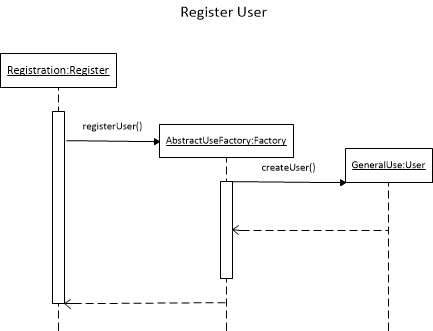
\includegraphics[width=\textwidth]{fortran-design-srs/images/Register_User_Sequence_Diagram.png}
      \caption{Register User Sequence Diagram}
    \end{figure}
    
    \clearpage
    
    \begin{figure}[h!]
      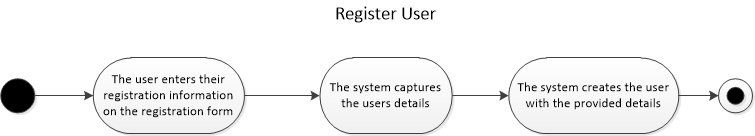
\includegraphics[width=\textwidth]{fortran-design-srs/images/Register_User_Activity_Diagram.png}
      \caption{Register User Activity Diagram}
    \end{figure}
    
    \begin{figure}[h!]
      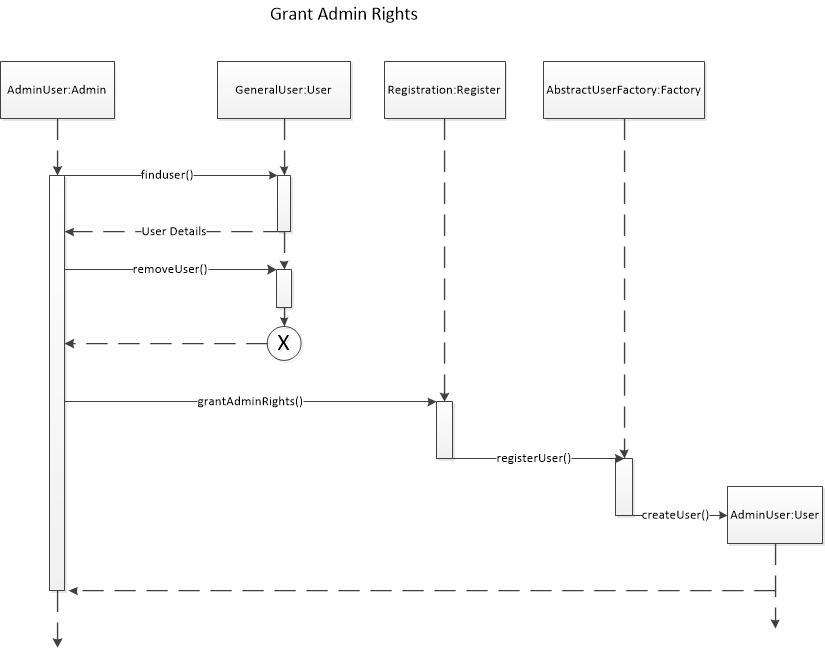
\includegraphics[width=\textwidth]{fortran-design-srs/images/Grant_Admin_Rights_Sequence_Diagram.png}
      \caption{Grant Admin Rights Sequence Diagram}
    \end{figure}
    
    \begin{figure}[h!]
      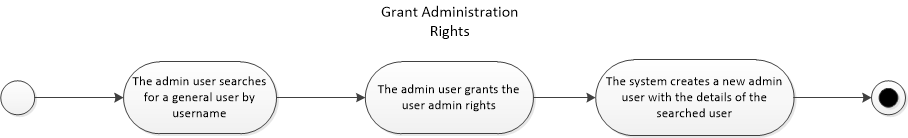
\includegraphics[width=\textwidth]{fortran-design-srs/images/Grant_Admin_Rights_Activity_Diagram.png}
      \caption{Grant Admin Rights Activity Diagram}
    \end{figure}
    
    \begin{figure}[h!]
      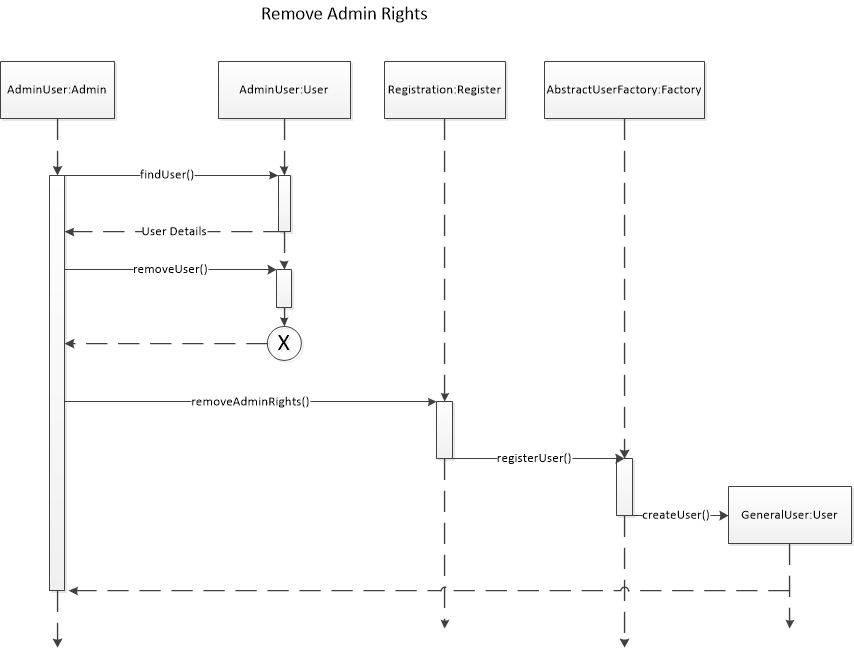
\includegraphics[width=\textwidth]{fortran-design-srs/images/Remove_Admin_Rights_Sequence_Diagram.png}
      \caption{Remove Admin Rights Sequence Diagram}
    \end{figure}
    
    \begin{figure}[h!]
      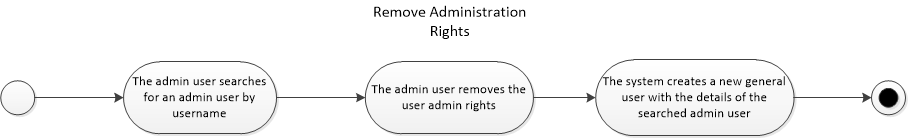
\includegraphics[width=\textwidth]{fortran-design-srs/images/Remove_Admin_Rights_Activity_Diagram.png}
      \caption{Remove Admin Rights Activity Diagram}
    \end{figure}
    
    \clearpage
    
\subsection{Notifications}
\subsubsection{Scope}
 The notifications module provides notifications to system users regarding
    particular system updates that a user would like to be notified about through
    some medium external to the application.
    
    \begin{figure}[h!]
        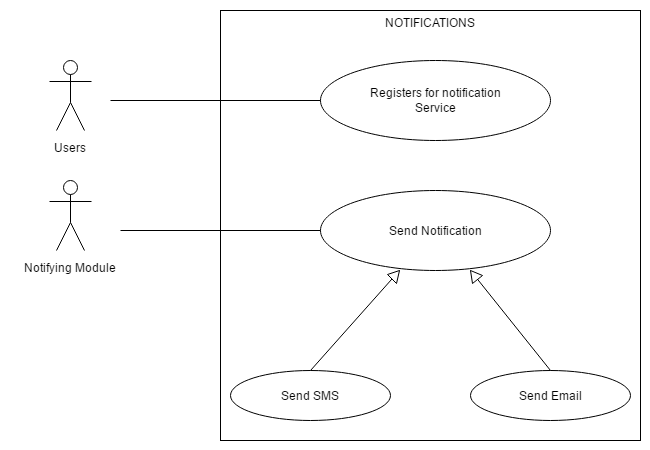
\includegraphics[width=\textwidth]{fortran-design-srs/images/Notifications_Use_Case.png}\caption{Notification Use Case Diagram}
    \end{figure}
 
\clearpage

\subsubsection{Design details}
   
    \begin{figure}[h!]
      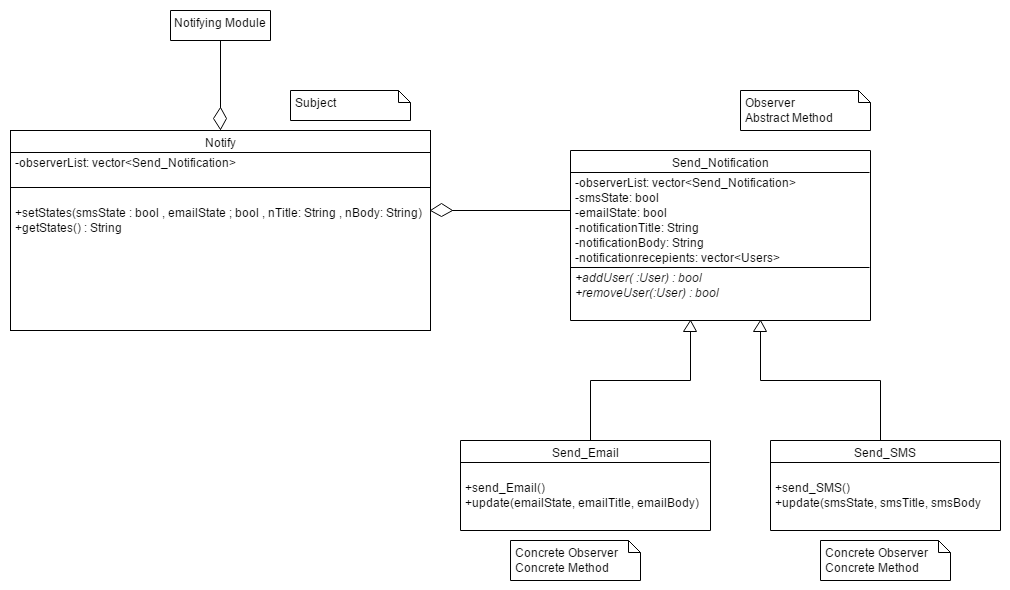
\includegraphics[width=\textwidth]{fortran-design-srs/images/Notifications_Class_Diagram.png}\caption{Notification Class Diagram}
    \end{figure}
    
    
    \begin{flushleft}
    
        For the notifications subsystem the observer design pattern came to light. This pattern allows objects to change state and all of its dependents follow suit. This allows a notification state to be used that can update whether or not a notification needs to be sent out. In this case the push method of observer was used. Also evident is the template design pattern that uses the concrete observers to redefine the way in which the notifications are sent. Notifying modules are also given the flexibility to decide which medium(s) are used for the notification. Any notifying module can call the setState() method to initiate the sending of a notification. This function will allow for boolean values to be passed to the sending classes to clarify which notification method/s are to be used. Included in this method are variables to encompass the title and body of the notification. The notify class would then call the notify method which in turn would call the update() functions on the concrete observers and that would trigger the sending of the notifications.  
        
        \bigskip

        
        There are methods in the Send Email and Send SMS classes that allow users to be added to the user lists for the notifications to either or both of these mediums. There is also provision for more notification mediums to be added in the future and these can be attached to the Notify class. Should a notification medium be unavailable it can be detached from the Notify class until it is available. The Notify class can be called from any other module that would like to request a notification to be sent out to users which allows for modularity.
        
        
        \clearpage

        Notify: Subject
        

        Send Notification: Observer(Observer) / Abstract Method(Template)
        

        Send Email: Concrete Observer1(Observer) /Concrete Method(Template)
        

        Send SMS: Concrete Observer2(Observer) / Concrete Method(Template)
    
    \end{flushleft}
    
    \mbox{}\\
    \bigskip
  
    
    \begin{figure}[h!]
        \includegraphics[width=\textwidth]{fortran-design-srs/images/Notification_Sequence_Diagram.png} \caption{Notification Sequence Diagram}
    \end{figure}
  
    
    \mbox{}\\
    \bigskip
    
    
    \begin{figure}[h!]
        \includegraphics[width=\textwidth]{fortran-design-srs/images/User_Register_Notification.png} \caption{Add User Activity Diagram}
    \end{figure}
    
    
    \mbox{}\\
    \bigskip
    
    \begin{figure}[h!]
        \includegraphics[width=\textwidth]{fortran-design-srs/images/Notifications_Activity_Diagram.png} \caption{Send Notification Activity Diagram}
    \end{figure}
    
    
    \mbox{}\\
    \bigskip
    \clearpage
    
    \begin{figure}[h!]
        \begin{center}
            \includegraphics[width=0.6\textwidth]{fortran-design-srs/images/Notification_State_Diagram.png} \caption{Notification State Diagram}
        \end{center}
    \end{figure}
    
    \mbox{}\\
    \bigskip
    \newpage
    
\subsection{Events}
\subsubsection{Scope}
    The events module serves as the system to log, update and view events that might be hosted on the University. These events include Educational and Social events, but can be branched out to other categories as they arise.
    
    \begin{figure}[h!]
        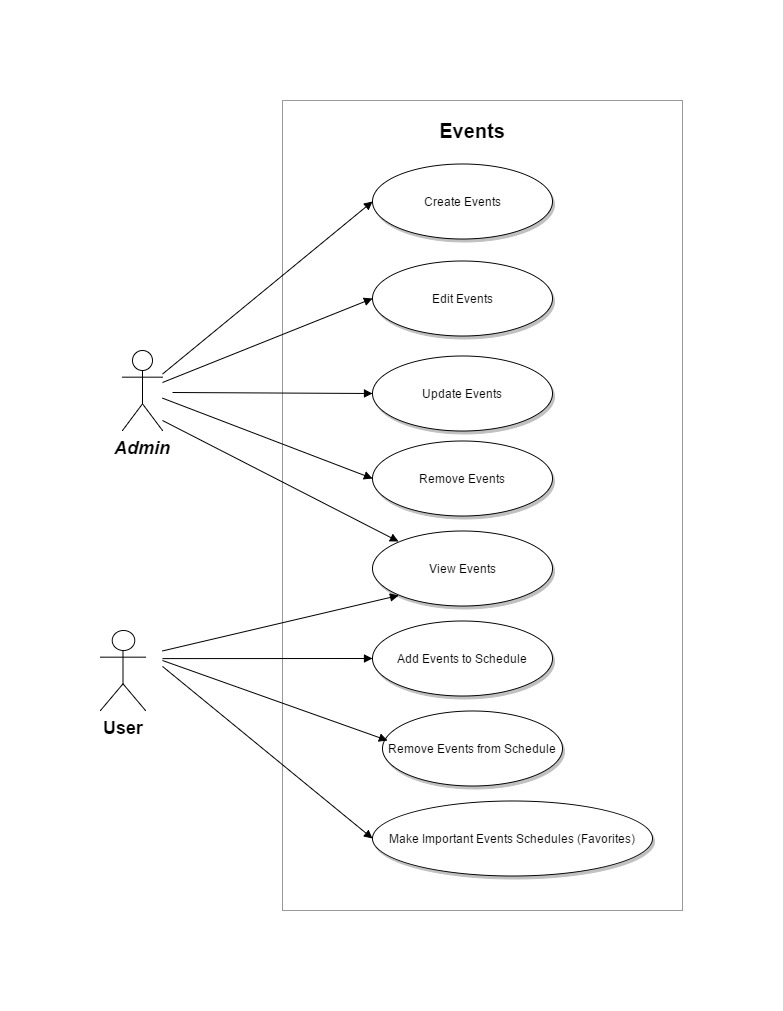
\includegraphics[width=0.8\textwidth]{fortran-design-srs/images/EventUC.jpg}
        \caption{Events Use Case Diagram}
    \end{figure}
 
\clearpage

\subsubsection{Design details}
   
    \begin{figure}[h!]
      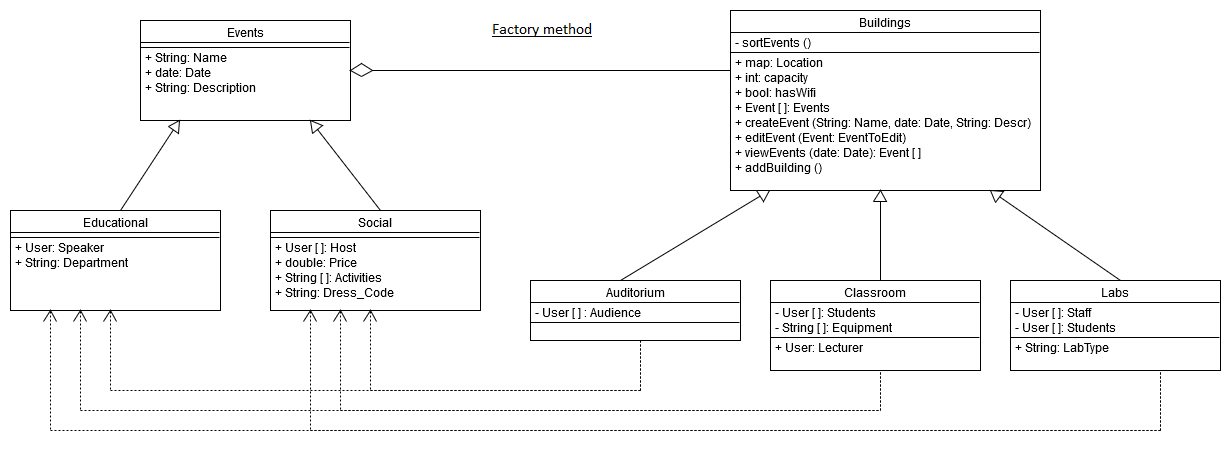
\includegraphics[width=\textwidth]{fortran-design-srs/images/ClassDiagramEvents.png}
      \caption{Events Class Diagram}
    \end{figure}
    
    
    \begin{flushleft}
    
        For the events subsystem the Factory Method design pattern is applicable, as this pattern allows objects of the same abstract type to be initiated by letting a certain Creator or object user decide which type of concrete class to instantiate.
        
        \bigskip
        
        In this instance, a certain type of building is allowed to host an event of a certain type. This allows for greater accuracy in searching for a certain event in a certain building. It also enables the events to be easily sorted and ordered to make presentation to the user easier. The fact that buildings as well as events can be created or altered dynamically also is catered for by the Factory Method, since a concrete building can easily be created and linked to the relevant concrete event, which can also be created and destroyed with ease. This is done while still maintaining the relevant needed information and functionality that each building and event needs (which is hosted in the abstract class).
        
        \bigskip
        
        There are methods in the Buildings class that allow users to add buildings as they are needed. The Buildings class also allows users to edit, view or add Events. This is done in the Building class as it is implemented with the Creator role of the design pattern. The viewEvents() function will act as a searcher function that will traverse the list of events that the relevant building is hosting in order to enable a user to invoke other functionalities, like  viewing an event or editing an event. The Buildings class can be called from any other module that would like to have access a to Events, like if the User class wants to add an event.
        
        \bigskip
        Design Pattern Entities:
        \bigskip
        
        Buildings: Creator
        \newline
        Auditorium: Concrete Creator
        \newline
        Classroom: Concrete Creator
        \newline
        Labs: Concrete Creator
        \newline
        Events: Product
        \newline
        Educational: Concrete Product
        \newline
        Social: Concrete Product
    
    \end{flushleft}
    
    \mbox{}\\
    \bigskip
  
    
    \begin{figure}[h!]
        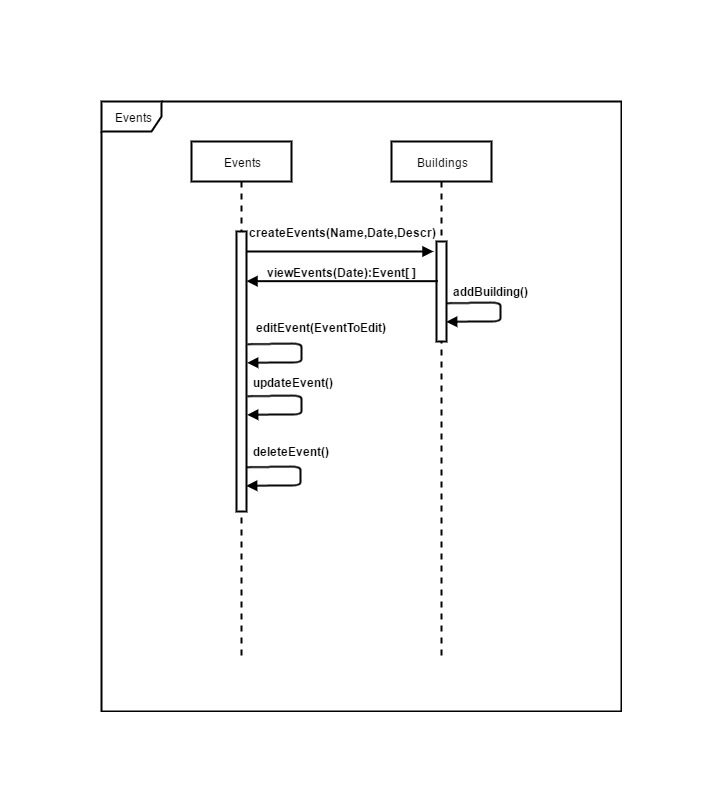
\includegraphics[width=\textwidth]{fortran-design-srs/images/EventsSequence.jpg} \caption{Events Sequence Diagram}
    \end{figure}
  
    
    \mbox{}\\
    \bigskip
    
    
    \begin{figure}[h!]
        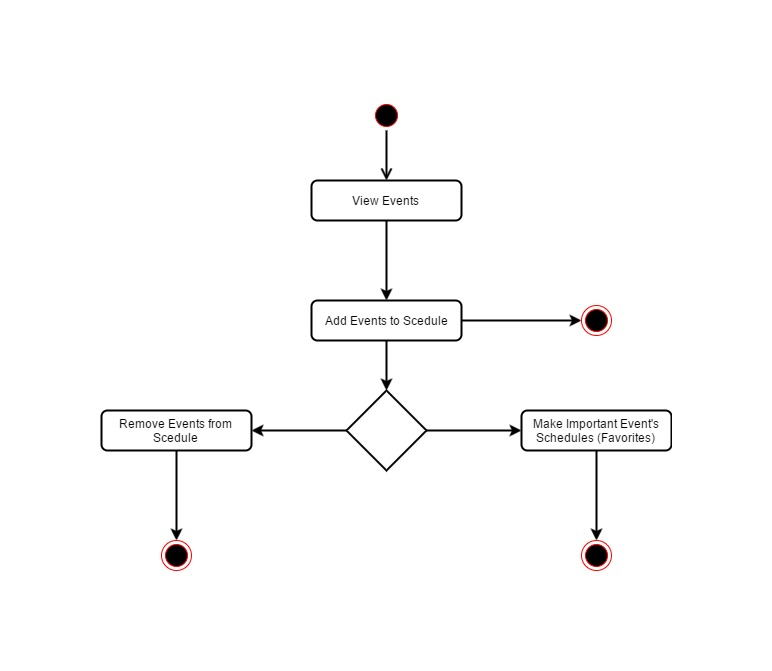
\includegraphics[width=\textwidth]{fortran-design-srs/images/ActivityDiagramUser.jpg} \caption{Normal User Activity Diagram}
    \end{figure}
    
    
    \mbox{}\\
    \bigskip
    
    \begin{figure}[h!]
        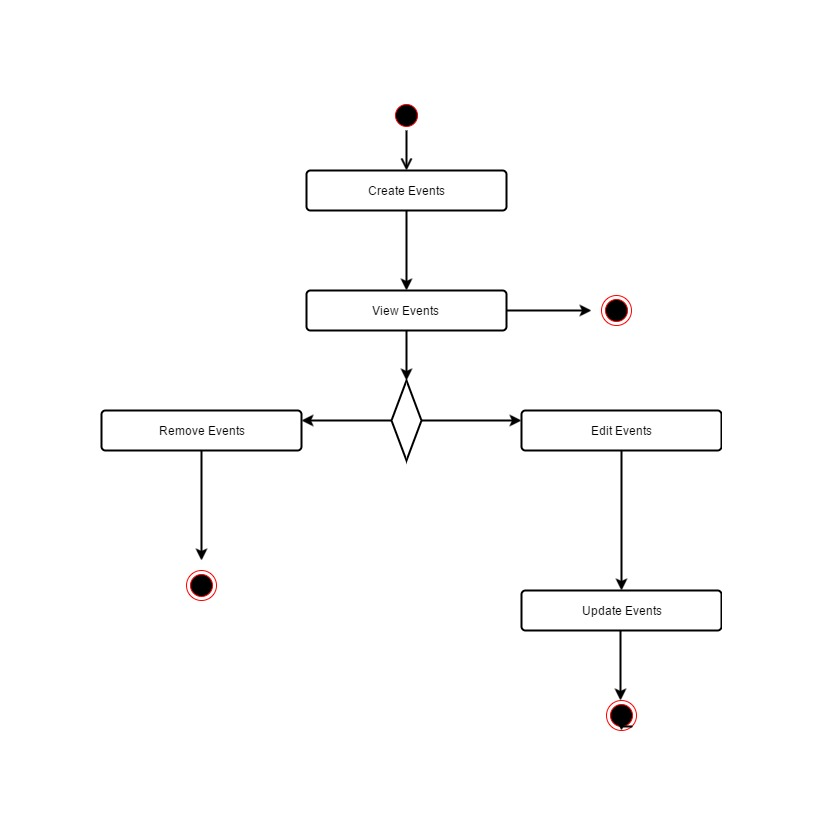
\includegraphics[width=\textwidth]{fortran-design-srs/images/ActivityDiagramAdmin.jpg} \caption{Advanced User Activity Diagram}
    \end{figure}
    
    
    \mbox{}\\
    \bigskip
   
    
    \begin{figure}[h!]
        \begin{center}
            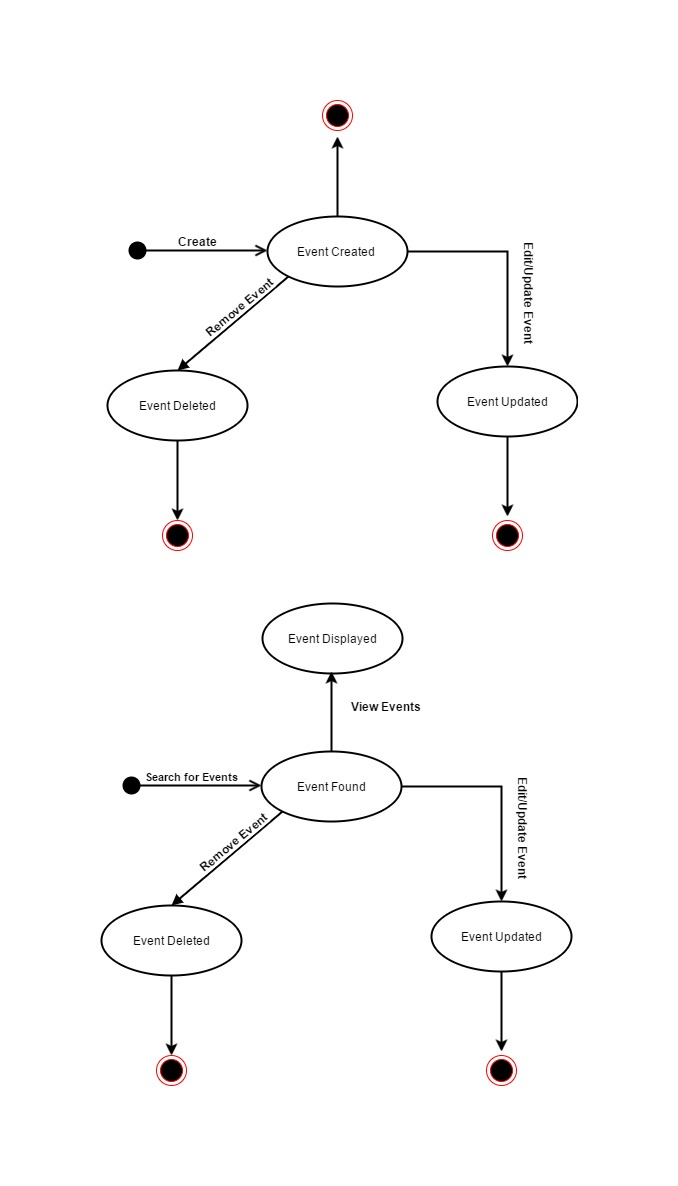
\includegraphics[width=0.6\textwidth]{fortran-design-srs/images/StateDiagramEvent.jpg} \caption{Events State Diagram}
        \end{center}
    \end{figure}
    
    \mbox{}\\
    \bigskip
    \clearpage
    \newpage
    
\subsection{Points Of Interest}
\subsubsection{Scope}
This subsystem services to gather, maintain, persist and provide information related to the locations, this includes both private and public information. The Admin is allowed to create, and update and delete locations in the system whereas all other users are only allowed to view(read) the locations.
A pin is dropped to signify location, and named as that specific location is saved for future reference. The system displays saved pins as well as allows for details about pins to be edited by admin. Admin can also delete pins from saved locations. Furthermore, locations specified for pins are acquired using services provided by the GIS module.

\mbox{}\\
    \bigskip
    
\begin{figure}[h!]
        \begin{center}
            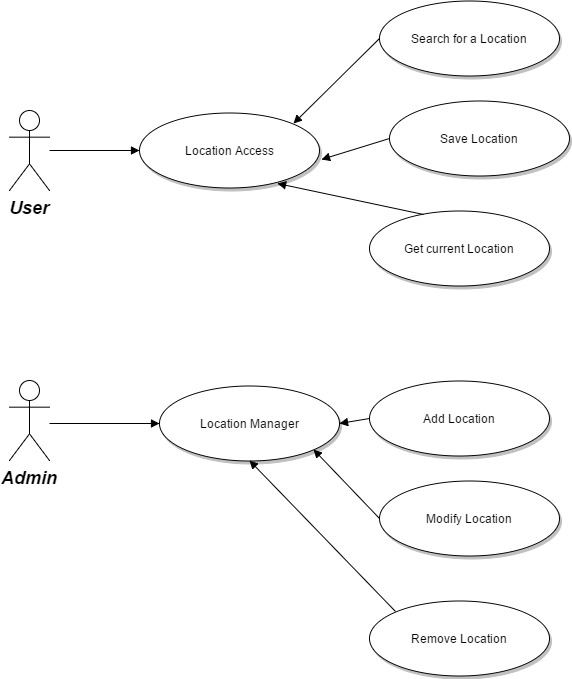
\includegraphics[width=0.6\textwidth]{fortran-design-srs/images/POI_Use_Case_Diagram.jpg} \caption{Points of Interest Use Case Diagram}
        \end{center}
    \end{figure}
    
\newpage
\subsubsection{Design details}

\begin{figure}[h!]
        \begin{center}
            \includegraphics[width=1.0\textwidth]{fortran-design-srs/images/class_diagram.png} \caption{Points Of Interest Class Diagram}
        \end{center}
    \end{figure}

The appropriate design pattern applicable for the Points Of Interest Subsystem is the Facade design pattern. This Structural design pattern encapsulates the complex database containing information about the various buildings and points of interests within this subsystem. The user need not require the knowledge of the locations management system but only access each location.
\newline 
\noindent In this case, the Points of Interest class acts as a Facade to the regular user, providing them with an interface to view, select and save a desired locations, or Points of Interest, however, not allowing the user access to create, update or delete any locations as that is only authorized by the Admin user.
\newline \newline
\noindent Design Pattern Entities:
\begin{itemize}
\item Client - Regular User
\item Facade - Points of Interest
\item Additional Facade - Location Manager
\end{itemize}

\mbox{}\\
    \bigskip
\begin{figure}[h!]
        \begin{center}
            \includegraphics[width=1.0\textwidth]{fortran-design-srs/images/sequantial_Diagram.png} \caption{Points of Interest Sequential Diagram}
        \end{center}
    \end{figure}

\mbox{}\\
    \bigskip
    
    \begin{figure}[h!]
        \begin{center}
            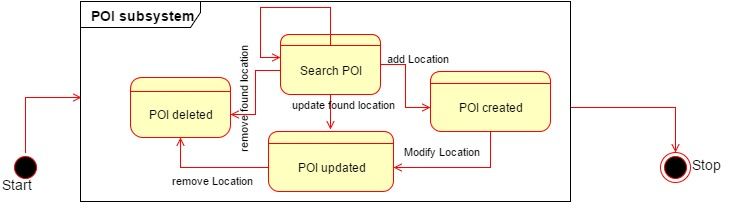
\includegraphics[width=0.6\textwidth]{fortran-design-srs/images/POI_State_Diagram.jpg} \caption{Points Of Interest State Diagram}
        \end{center}
    \end{figure}
    \mbox{}\\
    \bigskip
    \clearpage
\newpage
\section{System Design}
An overarching view of the whole NavUP system is shown in the deployment diagram below. This describes the relation between subsystems(core and add-ons) as well as the additional subsystems identified for the system. All components describe their relational functions to operate the system, NavUP.
\mbox{}\\
    \bigskip
\begin{figure}[h!]
	\begin{center}
		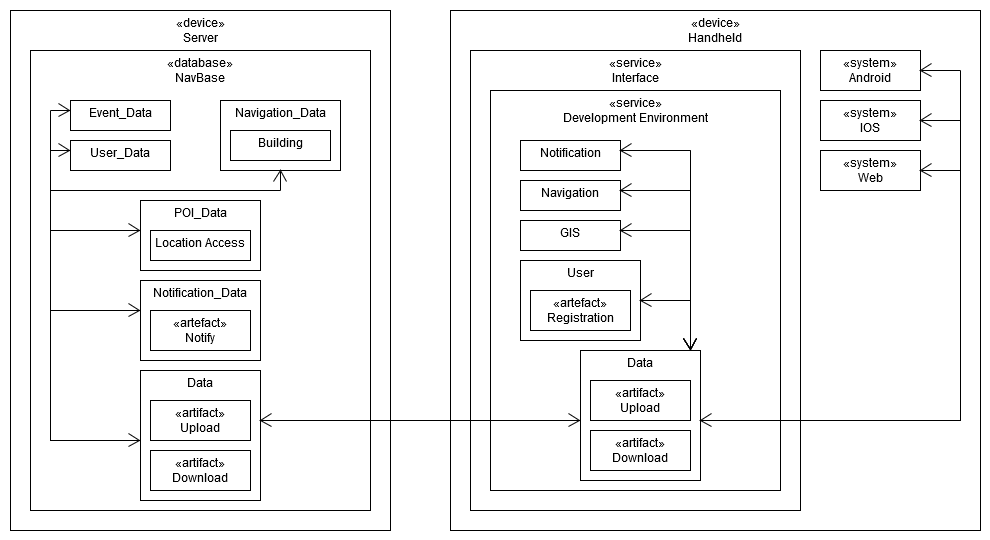
\includegraphics[width=1.2\textwidth]{fortran-design-srs/images/DeploymentDiagram.png} \caption{Deployment Diagram of NavUP system}
		\end{center}
\end{figure}
\mbox{}\\
    \bigskip
    
    
    \clearpage
\newpage

\section{Other Non-functional Requirements}
\subsection{Performance Requirements}
The notifications will have to be pushed out in a timely manner such that the time between creation and time of sending of notifications is minimal.
\newline
The system will also have to handle sending bulk e-mails and SMS's from multiple notifying modules in a manner that will not cripple the system or put the system at risk.
\newline
The system must accommodate any number of users at any given time period. All page requests must be processed by the system in no more than the average response time of the Internet connection. 
\newline
The system must display confirmation of user log ins, as well as display favorite Points of Interest relative to the user profile.
\newline
The user interface should have fast response times. The application should take too long to load another interface upon the user's request.
\subsection{Design Constraints}

\begin{flushleft}
    Notifications should not be long such that loading times are affected(e-mail) or that partitioning of messages occurs(SMS). Notifications should be pushed out within a given time frame. Notifications should conform to the rules of the medium of transport. No unnecessary data/information should be sent in these notifications. 
\newline
    The design of the system must take into consideration the amount of space which the application will occupy on the user's device. The application itself should ideally not exceed 40mb. The system should also be able to cater for low end devices which may not have a substantial amount of computational power. The application should use no more than 32mb of ram.
    \end{flushleft}

\subsection{Software System Attributes}
\subsubsection{Reliability}    
    \begin{flushleft}
    If an error occurs within the system, an appropriate error message should always be displayed. For example, if the registration of a user fails because a user with the same information and credentials has already been registered, the system should notify the user that the user with the provided credentials has already been registered.
\bigskip

    The notifications subsystem is crucial in informing users of possible information. With this it is of utmost importance that all notifications sent are received by the registered users.
    \end{flushleft}
    
    	\subsubsection{Availability}    
    \begin{flushleft}
    The system must be reliable in terms of up time. All of the system functionality should always be readily available.
    \end{flushleft}
    
    	\subsubsection{Security}    
    \begin{flushleft}
    Notifications and communications must be secure such that no malicious activity occurs on the system and users are not conveyed wrong information. In addition to this the users data must be kept in a secure environment so as to prevent any "leaking" of their personal information.
    \end{flushleft}
    
    	\subsubsection{Maintainability}    
    \begin{flushleft}
    The amount of notification mediums is increasing and to accommodate this new forms of communication mediums must be easily appended to the system.
    \end{flushleft}
     \clearpage
     
\subsection{Technology choices}
Below is a summary of the technology choices for the NavUp system and a brief motivation for them.
\begin{itemize}
  \item TCP/IP - We chose the TCP protocol for information transfer between the server and devices as this method allows for error checking in data and using this we can confirm that the user has received the data/information that was sent.
  \item PostgreSQL - This would be the database management system used for the system, this platform has features such as providing extensibility in which we can customize it to the needs of the system.  Using a separate platform for the database allows it to be separated from the rest of the system. 

\item PostGIS - Integrating this feature will allow the GIS system to communicate directly with the database system allowing easier integration with location management. PostGIS adds additional types to the database such as geometry, geography, raster and others. This feature will also allow for both processing and analytic functions to be applied for both vector and raster data.
\item Traccar - This is a open source GPS tracking platform that will be used to allow tracking on all devices. This service provides client side tracking as well as server side management with location reports done in real time. The client is available for iOS and Android which suits our needs. Traccar also supports multiple communication protocols. 
\item HTML5 - HTML5 is a markup language used for creating websites and this will be used for the Web UI of the NAVUP system. This has been chosen because it allows for a variety of integrations and allows for the structure of the web pages to be consistent. 
\item BOOTSTRAP - This is an add-on for the HTML5 platform that serves as a template for creating webpages easily. The included functions and design attributes could be useful in creating the Web UI.
\item Ekahau HeatMapper - This is a networking facility that allows the use of wireless network routers to locate devices and analyse their distances from various wireless points. This will enable us to generate a heatmap of the campus as well as pinpoint the location of devices dependent on the wifi signal strength that they receive.
\item CSS - Cascading Style Sheets will be used to allow a design template to be applied to the HTML5 webpages that will allow for the design to be consistent among all of them.
\item PHP - Hypertext Preprocessor is a scripting language that will be used alongside(embedded in) HTML5 to allow server side scripting. This allows the code part of the system to be more secure and allow information to be sent to and from the server in a secure way.
\item Google Maps - Google Maps will be used to aid the navigation process within the application so that coordinates can be sent to the server for processing on the UP Campus Map. 
\end{itemize}

\end{document}